\documentclass[doktyp=semarbeit, sprache=german]{TUBAFarbeiten}
\usepackage[utf8]{inputenc}
\usepackage[T1]{fontenc}
\usepackage{graphicx} 
\usepackage{amsmath}
\usepackage{subcaption}
\usepackage{booktabs}
\usepackage{url}
\captionsetup{compatibility=false}
\bibliographystyle{unsrt}
\TUBAFFakultaet{Fakultät für Maschinenbau, Verfahrens- und Energietechnik}
\TUBAFInstitut{Institut für Automatisierungstechnik}
\TUBAFTitel[Moderne Methoden der Bildverarbeitung am Beispiel Gesichtserkennung]{Moderne Methoden der Bildverarbeitung am Beispiel Gesichtserkennung}
\TUBAFUntertitel{Anwendung von Informations- und Automatisierungssystemen}
\TUBAFBetreuer{Prof. Andreas Rehkopf}
\TUBAFAutor[S. Dressel und H. Krumbiegel]{Samuel Dressel und Hannes Krumbiegel}
\TUBAFDatum{\today}
\begin{document}
\maketitle
\tableofcontents
\newpage
\section{Einleitung}
\section{Grundlagen}
Einführend zum besseren Verständnis des Themenkomplexes ist es wichtig, einige wesentliche Begriffe zu definieren und außerdem voneinander abzugrenzen. Zunächst gilt es, zwischen der Lokalisation eines Gesichtes an sich und der Zuordnung des Gesichts zu einer bestimmten Person zu unterscheiden. Im ersten Fall wird geprüft, ob und wo ein Gesicht zu sehen ist, im zweiten, um wen es sich handelt \cite{FaceRecognitionWikipedia}. Wir sprechen somit zum einen von der Gesichtserkennung und zum anderen von der Gesichtsidentifizierung. Im englischen Sprachgebrauch unterteilt man den Teil der Gesichtsidentifizierung zusätzlich noch in eine menschliche Erkennung (\textit{face perception}) und in eine maschinelle Erkennung (\textit{face recognition}). In dieser Arbeit wird sich jedoch lediglich auf die maschinelle Gesichtsidentifizierung beschränkt.
\section{Gesichtserkennung (Face Detection)}
\section{Gesichtsidentifizierung (Face Recognition)}
Das Gebiet der Gesichtsidentifizierung umfasst alle Methoden und Techniken, mit der es möglich ist, basierend auf visuellen Material Menschen eindeutig zu identifizieren. Die Gesichtsidentifizierung baut dabei auf der Gesichtserkennung auf. Insbesondere in den letzten Jahren wurden nach und nach zahlreichen Algorithmen und Methodiken entwickelt, um Gesichter maschinell zu identifizieren. Insbesondere im Hinblick auf die Automatisierung der Gesichtsidentifizierung stellt erst das Jahr 1973 den Startpunkt dar, als Takeo Kanade in seiner Dissertation das erste automatisierte System zur Gesichtsidentifizierung vorstellte \cite{Takeo}. Jedoch konnte grade aufgrund der begrenzten Rechenleistung zu dieser Zeit dieses System noch längst nicht effizient arbeiten. Ein wesentlicher Fortschritt wurde erst im Jahr 1990 durch die Forscher Kirby und Sirovich erzielt, welche die Hauptkomponentenanalyse (Karhunen-Loève-Transformation) verwendeten \cite{Kirby}. Hierbei wird eine Vielzahl von generierten Variablen auf eine geringe Zahl aussagekräftiger Parameter reduziert. Dadurch wird gleichzeitig auch die Komplexität und der Rechenaufwand verringert. Weiterhin stellte die Arbeit von Matthew Turk und Alex Pentland einen weiteren Meilenstein dar, welche sogenannte Eigengesichter (Eigenvektoren) zur Gesichtsidentifizierung nutzten \cite{Turk}. Diese Techniken werden auch noch in den derzeitigen State of the Art Methoden genutzt.
\\\\Im Folgenden soll auf eine Reihe dieser Methoden und Herangehensweisen eingegangen, einige Anwendungsbeispiele genannt und die Problematiken der Gesichtsidentifzierung thematisiert werden.
\subsection{Methoden der Gesichtserkennung}
Grundlegend können alle Methoden der Gesichtsidentifizierung in zwei wesentliche Schritte eingeteilt werden. Der erste Schritt ist die Extraktion und Selektion von Merkmalen aus dem visuellen Input; der zweite Schritt stellt die Klassifizierung der Merkmale dar \cite{FRS}. Desweiteren können Techniken zur Gesichtsidentifizierung in die Art der verwendeten Merkmale unterteilt werden. Diese können entweder geometrische Features sein (Form der Augen, Position der Nase, ...) oder fotometrische Features sein (Texturen, Farbwerte, ...).
\subsubsection{Hauptkomponentenanalyse (PCA) mit Eigengesichtern}
Das erste Verfahren, welches im Rahmen dieser Ausarbeitung näher betrachtet werden soll, ist die Hauptkomponentenanalyse (Principal Component Analysis, PCA) mit Eigengesichtern. Die Idee der Gesichtsidentifizierung mit PCA ist es, vorhandenes Bildmaterial so zu reduzieren, dass es sich für eine Auswertung eignet, ohne dabei die wesentlichen Merkmalsinformationen zu verlieren \cite{PCANova}. Man spricht hier von einer Dimensionsreduzierung. Die Hauptkomponentenanalyse an sich beinhaltet noch nicht den kompletten Prozess der Gesichtsidentifizierung, sondern stellt vielmehr ein Tool dar, welches von finalen Methoden im ersten Schritt der Selektion genutzt wird. Dies ist vor allem im Hinblick auf die Effizienz dieses Prozesses von großer Wichtigkeit.
\begin{figure}
\captionsetup[subfigure]{justification=centering}
\centering
\begin{subfigure}[c]{0.49\textwidth}
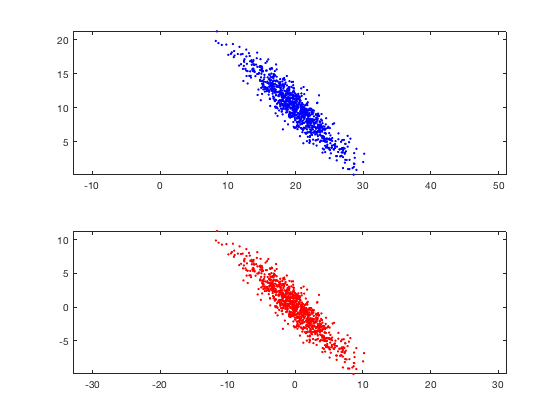
\includegraphics[width=1\textwidth]{images/PCA1.png}
\subcaption{Zweidimensionale Punktewolke - beide Datensätze sind identisch mit dem Unterschied, dass das rot gefärbte Diagramm nullzentriert ist}
\end{subfigure}
\begin{subfigure}[c]{0.49\textwidth}
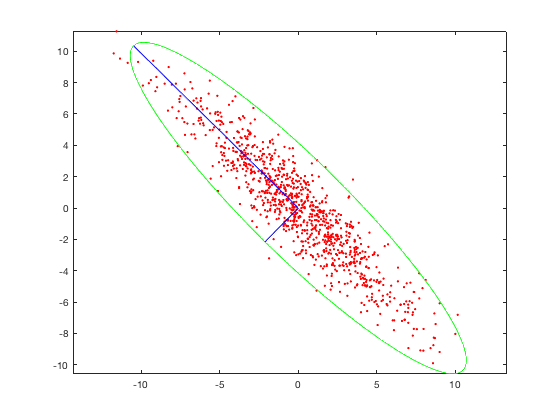
\includegraphics[width=1\textwidth]{images/PCA2.png}
\subcaption{Durch Bestimmung der Eigengesichter generierte Achsen; die längere der beiden blauen Achsen stellt dabei die Achse mit einer maximalen Streuung der Daten da, wenn die Punktewolke auf diese projiziert wird}
\end{subfigure}
\caption{Reduzierung der Dimension einer zweidimensionalen Punktewolke }
\label{img:PCA}
\end{figure}Um die Funktionsweise der Hauptkomponentenanalyse mit Eigengesichtern zu verstehen, kann man sich die einzelnen Merkmale als zweidimensionale Punktewolke vorstellen (Abbildung \ref{img:PCA}a). Eine Dimensionsreduzierung wird den Datensatz in diesen Fall von einer zweidimensionalen Ebene in eine eine eindimensionale Ebene transformieren \cite{PCAPython}. Wie auch bei allen anderen Algorithmen zur Dimensionsreduzierung geschieht dies im Fall der Hauptkomponenentenanalyse durch das Finden einer Hyperebene, auf welche die einzelnen Punkte projiziert werden können. Bei der Hauptkomponentenanalyse wird die Hyperebene so gewählt, dass bei einer Projektion alle Punkte eine maximale Streuung erzielen. Es wird sozusagen die Achse der maximalen Varianz gesucht. Im Fall der Punktewolke in Abbildung \ref{img:PCA} ist dies die längere blaue Linie. Um diese Linie zu finden, kommen nun die sogenannten Eigengesichter zum Tragen. Diese Eigengesichter sind nichts anderes als die Eigenvektoren der Kovarianzmatrix der gegebenen Datenmenge. Da in dem Fall der Hauptkomponentenanalyse die Achsen der maximalen Varianz generiert werden, werden die wichtigsten Informationen aus der Menge von Merkmalen erhalten. Für den zweiten Schritt der Klassifizierung im Rahmen der Gesichtsidentifizierung wirkt sich eine große Streuung zusätzlich positiv aus.
\subsection{Kritik und Probleme}
Die Thematik der Gesichtsidentifizierung im Vergleich zu einer lediglichen Gesichtserkennung im Sinne der Unterscheidung von anderen Objekten bringt eine Vielzahl von neuen Problemen mit sich. Und dies längst nicht nur auf der technischen Seite, sondern auch im Hinblick auf ethische Aspekte.
Betrachtet man die auftretenden Probleme der technischen Umsetzung, so können unterschiedliche Herausforderungen durch die Verwendung von unterschiedlichen Methoden und Technologien gemeistert werden. Jedoch werden bestimmte Schwierigkeiten noch längst nicht vollständig gelöst. Klassische Methoden, welche ihren Input aus klassischem Bildmaterial beziehen, haben mit einer Reihe ganz unterschiedlicher Probleme zu kämpfen \cite{MainBook}:
\begin{itemize}
\item Viele zweidimensionale Methoden liefern nur verwendbare Ergebnisse unter ausreichend guten Lichtverhältnissen. Auch ein großer Kontrast bzw. Variation der Beleuchtung kann die Effizienz dieser Methoden erheblich einschränken.
\item Die Verdeckung insbesondere der oberen Gesichtsareale durch eventuelle Gadgets wie Brillen, Hüte oder Kapuzen verringert die Genauigkeit oder kann eine Gesichtsidentifizierung nahezu unmöglich machen. Abhilfe schafft hier die Verwendung von Wärmesignaturen zur Gesichtsidentifzierung.
\item Klassische Verfahren, die auf die Textur bzw. die Form des Gesichts zur Identifizierung angewiesen sind, funktionieren nur, wenn ein ausreichend optimaler Blickwinkel auf das Gesicht gegeben ist.
\item Bei der Identifizierung von Menschen muss der natürliche Alterungsprozess und damit die Veränderung des Gesichts als ein negativer Faktor beachtet werden. Dies erfordert entweder eine aktuelle Vergleichsdatenbank oder das Verwenden einer hinreichend gute KI, um den Alterungsprozess des Gesichts abbilden zu können.
\end{itemize}

\section{Zusammenfassung und Ausblick}
\newpage
\bibliography{literatur}{}
\addcontentsline{toc}{section}{Literatur} 
\end{document}